\section{Transactions}
\subsection{Overview}

\begin{figure}[H]
    \centering
    %\includegraphics[width=6.5in,height=2.75in]{media/image14.jpg}
    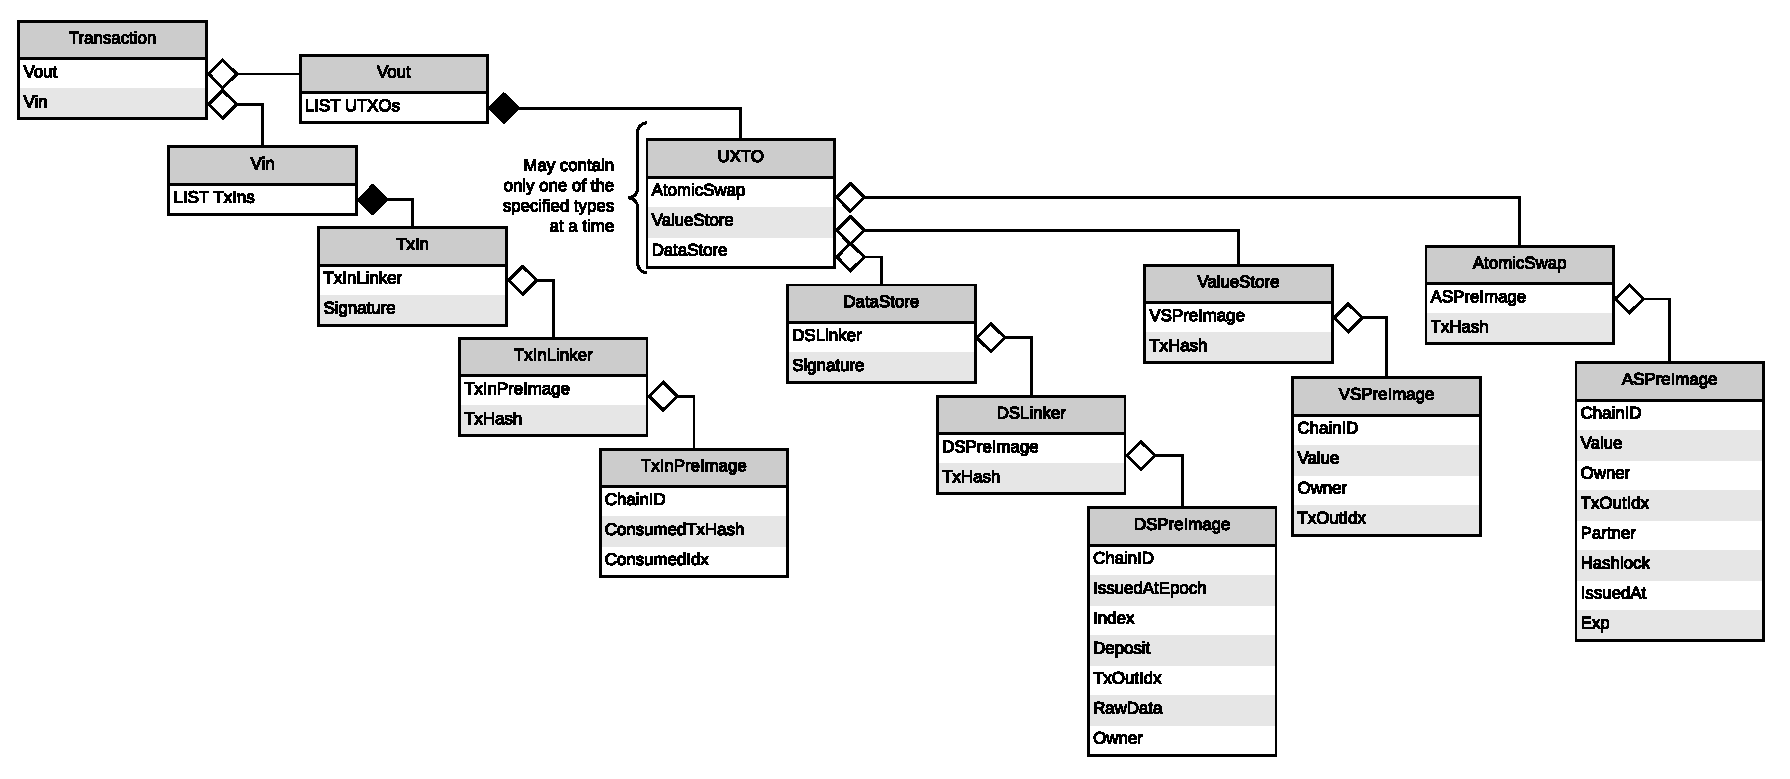
\includegraphics[scale=0.5]{figures/Transaction_Object_Primitive.pdf}
    \caption{Transaction Object Primitives}
\end{figure}


MadNetwork operates on a UTXO model that has many similarities to the
Bitcoin blockchain.
The divergence from the Bitcoin system is based on an attempt to
simplify the rules surrounding transaction validation.
Rather than integrate a scripting language, MadNetwork uses object
specific validation logic.
What this allows is a more efficient verification algorithm of pending
transactions as well as more granular proofs with respect to blockchain
state.

In the MadNetwork system, version numbers are not required at the
transaction level.
In the event that additional functionality is desired, new objects may
be created to accommodate such changes and the validation of such
objects may be treated as largely independent from the validation logic
of prior assumptions.
Thus updates to the protocol are purely additive modifications.
This choice was made based on the desire to build a system that is
resilient to the fact that it will require many years of continuous
uptime.


\subsection{The Transaction Object}

A transaction is composed of two top level fields.
These top level fields are vectors of objects.
The first vector, Vin, contains a vector of TxIn objects.
The second vector, Vout, contains a vector of UTXO objects.
A UTXO object must contain only one element from the mutually exclusive set of
allowed UTXO types.
These vectors are limited to 256 elements each and a transaction is limited to
a total of 3 megabytes max.
TxIn objects and UTXOs will be more fully covered in the following sections.

The operation of concern at the Transaction Object level is the mechanism by
which a transaction hash may be formed.
As may be seen above, every element of Vin and Vout contains a PreImage type as
the last element in the object hierarchy.
The PreImage objects define the protected parameters of a transaction.
In order to ensure that the process of transaction signing is secure, each
signed object must be immutably bound to the collection of input and output
objects.
This binding is done through the process of PreImage hashing.
The hashing of PreImage objects allows the formation of the TxHash value.
The full details of this operation will follow shortly.

Once a TxHash has been formed it may be injected into the appropriate layer of
all Vin and Vout objects.
For all signed objects, the TxHash is injected into a Linker object.
The canonical encoding of these Linker objects are what is signed for proof
of possession of an identified public key as the owner of a UTXO.
For all unsigned objects, the TxHash is injected into the top layer of the
object hierarchy.
This ultimately ensures protection against separation of the signature from the
intended action of the signer while also protecting against the known
transaction malleability attacks found in early versions of the Bitcoin
Protocol.
In order to provide more clarity around transaction hashing, the operation, in
detail, follows.
This example will utilize the TxIn object seen in the diagram above and speak
about UTXO objects in a generalized manner.

Before an explanation of the mechanics of TxHashing may be explained two
operations must be defined.
First, the concept of a UTXOID shall be explained.
Then the pseudoUTXOID shall be defined.

A UTXO may be identified by its UTXOID.
A UTXOID is created by hashing the concatenation of the TxHash that creates the
UTXO and the Vout index at which the UTXO was created.
MadNetwork enforces the assumption that there may never be two UTXO objects
that exist at the same time that are referenced by the same UTXOID.
This requirement is observed through the use of the StateTrie, which is covered
more thoroughly in other sections of this paper.
More formally:

\begin{align*}
    \text{idxBytes} &\coloneqq \text{uint32ToBigEndianBytes}(\text{idx}) \\
    \text{UTXOID} &\coloneqq \text{Keccak256}(\text{txHash}||\text{idxBytes})
\end{align*}

\noindent
The pseudoUTXOID, for a given UTXO, may be formed as follows:

\begin{align*}
    \text{idxBytes} &\coloneqq \text{uint32ToBigEndianBytes}(\text{idx}) \\
    \text{preImageHash} &\coloneqq \text{Keccak256}(\text{PreImage}) \\
    \text{pseudoUTXOID} &\coloneqq \text{Keccak256}(\text{preImageHash} ||
        \text{idxBytes})
\end{align*}

The operational explanation of TxHash formation may now begin.
Each TxIn object is composed of three layers.
The first layer is the TxIn object itself.
The first layer carries two fields.
The first field is the TXInLinker and the second field is the signature
of the canonical encoding of the TXInLinker.
The second layer is the TXInLinker.
The TXInLinker provides an intermediate layer such that the transaction
hash may be injected into the object.
The second layer contains two fields.
The first field is the TXInPreImage and the second field is the TxHash.
The third layer is the TXInPreImage.
This object codifies the UTXO being consumed through inclusion of the
ConsumedTxHash field and the ConsumedTxIdx field.
This hierarchy is also constructed on the UTXO objects found in Vout.

This topology allows for each PreImage layer of the transaction inputs
and outputs to be hashed concurrently.
Each of these hashes is then inserted into a Compact Sparse Merkle Trie
at a location defined by the type of object.
The resulting CSMT root hash is the TxHash.
For TxIn objects, this location is the UTXOID of the consumed UTXO and
the value is the hash of the TxIn PreImage.
For TxOut objects, the location is the pseudoUTXOID and the value is
the hash of the object PreImage.
Because a TxHash is not available to form the proper UTXOID of the
object, a pseudoUTXOID is used instead.

Once the TxHash is computed, each object from Vin and Vout has the
TxHash injected and all objects that must be signed are signed after
this injection.
This provides the means to immutably link a signature to a TxHash.

Unlike in Bitcoin, the sum of a Transaction’s input values must be
equal to the sum of a Transactions output values.
At this time, transaction fees are paid through the cleanup of stale
state.
Thus no direct mechanism to pay transaction fees is provided except
through explicitly naming a given validator or sending a UTXO to the
validator set using the validator’s Group Key.
The Group Key is a negotiated BLS key under a threshold cryptosystem.
This threshold cryptosystem will be explained more fully in the
consensus algorithm description.
Due to this threshold cryptosystem, the group of validators may
coordinate to distribute mining fees sent to the Group Key.
The authors of this paper are aware of the potential for an attack
against the storage of the system due to this design choice.
This attack is similar in nature to the DoS attacks on Ethereum that
occurred due to malicious transactions eating computation time.
In future versions of the protocol this attack may be trivially
mitigated through several mechanisms.
In the current implementation these attacks may be mitigated as well.
This protection is as follows.

If it is observed that an attack is ongoing, the validators may refuse
to mine any transaction that does not transfer value to the validator
set.
This is possible through the use of threshold cryptography that will be
covered in the consensus section of this paper.
The option that may be included in future versions is to allow a UTXO
to be formed that grants the miner the ability to consume the reward
directly or inject a key so the UTXO may be consumed later.
This has not been implemented at this time in order to simplify the
process of transaction processing.
Currently, the system mandates that all consumed objects must exist
prior to a transaction.
The system also requires that all transactions in a block do not
reference any object that any other transaction has already consumed.
Lastly, all objects in all transactions of a block must exist prior to
the block being mined.
These assumptions protect the atomicity of state transitions, but this
atomicity may be preserved with more complex handling of transaction
fees as an edge case.


\subsection{The TxIn Object}

\begin{figure}[H]
    \centering
    %\includegraphics[width=2.26in,height=1.69in]{media/image3.jpg}
    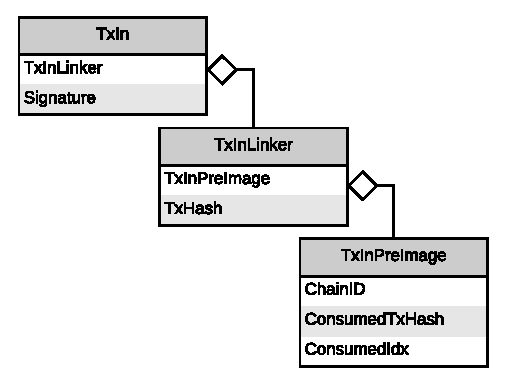
\includegraphics[scale=0.5]{figures/TxIn_Object.pdf}
    \caption{TxIn Object}
\end{figure}


A TxIn object allows a UTXO to be consumed by specifying the TxHash of
the Transaction in which the UTXO was formed and the index at which the
UTXO was created in the Vout vector.
All TxIn objects must be signed in order to prove possession of the
private key generated during object creation.
MadNetwork allows several pending transactions to reference the same
UTXO for consumption at a time through the utilization of an LRU-based
reference counting system.
A TxIn may not reference a UTXO created in the same transaction or
block.
As previously covered, this may be changed in future versions to allow
the edge case of mining fees.
All TxIn objects must point to either a known UTXO or a valid unspent
deposit from Ethereum.

In addition to consumption of MadNetwork UTXO objects, the TxIn object
may also cause the consumption of a Deposit from the Ethereum
blockchain.
Deposits into the sidechain may be triggered by any token holder on the
Ethereum blockchain.
These deposits become virtual UTXOs in the sidechain after a ten block
wait.
This process is controlled by a deposit smart contract on the Ethereum
blockchain.
Internal to this deposit contract there exists a monotonically
increasing counter.
For each deposit, this counter is incremented.
When a deposit is made, a hash is passed into the contract.
This hash is the hash of the public key that may be used to claim the
deposit on the sidechain.
The deposit itself will cause the associated tokens to be burned on the
Ethereum blockchain.
This action causes an event to be emitted that is observed by the
miners of the sidechain.
Once this deposit has matured for at least 10 blocks, it will become
available for use in the sidechain.
The deposit may be consumed by referencing the deposit in a TxIn object.
This reference may be formed by setting the consumedTxIdx field of the
TxIn object to the max value of uint32, setting the txHash to the big
endian uint256 equivalent of the counter at the time of the deposit,
and signing with the same private key as was used to create the public
key hash specified in the deposit contract invocation.
In order to prevent a deposit from being double spent, a permanent
record of having consumed the deposit is tracked in the State Trie of
the sidechain.
This tracking of state is permanent and allows the validators to not
perform any acknowledgment operations of a deposit having been spent
against the deposit smart contract.


\subsection{The DataStore Object}

\begin{figure}[H]
    \centering
    %\includegraphics[width=2.98in,height=2.28in]{media/image7.jpg}
    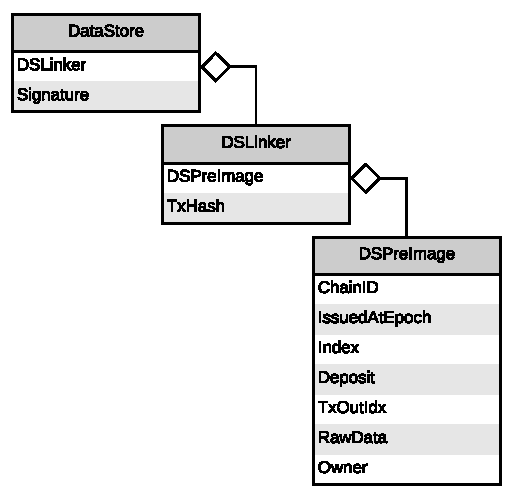
\includegraphics[scale=0.5]{figures/DataStore_Object.pdf}
    \caption{Data Store Object}
\end{figure}


A DataStore object is a type of UTXO.
This is the fundamental mechanism by which data may be stored in MadNetwork.
Rather than storing data in an account-based relationship, we selected
the use of a UTXO-based storage system to allow for a more traditional
atomic commitment mechanism as is readily available in database
technologies in general.
This capability allows a single transaction to consume many DataStore
objects and rewrite these objects in an atomic manner.
A DataStore is bound to a single epoch, where an epoch is a bounded
division of blocks in MadNetwork.
These divisions are deterministic and based on simple modulo operations.
The full specification of an epoch will be handled later in this paper.
Any transaction containing a DataStore must be included in the named
epoch of generation.
This constraint is manifest through the rent-based data storage
mechanisms employed by MadNet.
In addition to the actual data being stored, the deposit, the chainID,
the output index, the epoch of issuance, and the owner, each DataStore contains
an index.
The index allows a datastore to be referenced as a named element in the
virtual namespace defined by the hash of the public key of the
DataStore signer.
This index is built through a reference system in the database behind
the application, and this reference system enforces uniqueness of an
index in a given namespace.
This reference system allows $O(1)$ access to an element in a namespace.
There also exists an index that allows all objects in a namespace to be
traversed in $O(n)$ and $O(\log n)$ search may be implemented in future
versions of this system without impacting consensus.

\subsection{The ValueStore Object}

\begin{figure}[H]
    \centering
    %\includegraphics[width=1.75in,height=1.74in]{media/image1.jpg}
    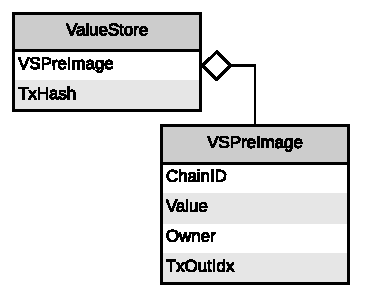
\includegraphics[scale=0.5]{figures/ValueStore_Object.pdf}
    \caption{Value Store Object}
\end{figure}



A ValueStore allows for the conveyance of MadNetwork tokens between
accounts in the MadNetwork and provides a mechanism for generating a
change output from a transaction.
The named owner is the only party that may consume a ValueStore object.
All value stores are also indexed according to the owner by default.
This allows iteration of UTXO objects for the purpose of simplifying
wallet software.
These objects are indexed in either smallest value to largest value and
may be iterated in forward and reverse.
This indexing allows efficient solutions of the knapsack problem using
greedy algorithms.
These greedy algorithms are not included in the logic of the node at
this time.
The inclusion of this index is intended to facilitate the minimization
of UTXO dust, as it is named in the Bitcoin context.


\subsection{The AtomicSwap Object}

\begin{figure}[H]
    \centering
    %\includegraphics[width=1.93in,height=2.23in]{media/image4.jpg}
    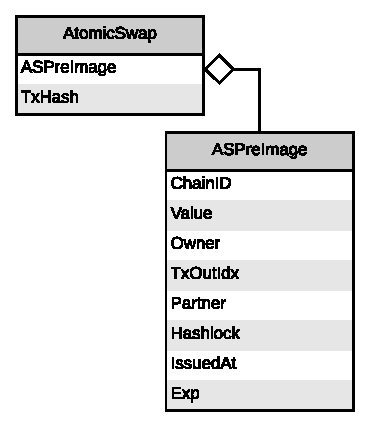
\includegraphics[scale=0.5]{figures/AtomicSwap_Object.pdf}
    \caption{Atomic Swap Object}
\end{figure}


Withdrawals from the sidechain occur through atomic swaps only.
This decision was made to dramatically reduce the complexity of the
protocol.
Since the primary utility of the underlying system is to write data
into the sidechain, and tokens are destroyed when such an event occurs,
this simplification reflects the intent of the system and allows the
amount of state that must be tracked to be dramatically reduced.
In this way the sidechain acts as a universal sink in the flow of
tokens.

The manner in which atomic swaps are facilitated is through the native
AtomicSwap object.
This object acts as a time-locked hash contract where time is measured
in epoch boundaries.
The safest manner in which to negotiate an atomic swap is for the
sidechain party to be the initial actor.
This pattern is also convenient because it allows an offer contract to
exist in the Ethereum EVM that orders may be matched against, and
MadNet was intentionally not built for complex smart contract
operations of this nature.

At the time of creation, any value stored in the AtomicSwap is locked.
During the time between issuedAt and exp, the partner may claim the
value stored in the AtomicSwap by revealing the preImage of the
hashlock.
The only party that may claim an AtomicSwap before exp is the partner
and only with a proof of knowledge of the hashlock-preimage.
If the AtomicSwap is not consumed before exp, any value stored in the
AtomicSwap will revert to owner.
Thus, only the partner or owner may consume this UTXO type.

The operational flow is as follows.
For the purpose of this explanation Mike will hold MadNetwork Tokens in
the MadNetwork itself and Erin will hold Ethereum in the EVM.
The protocol may begin once Mike and Erin are aware of each other's
desire to exchange, an exchange rate has been set, Mike has the hash of
Erin's public key that she will use in MadNetwork, and Erin has
Mike's Account he will use in Ethereum.

First, Mike will form a Transaction that transfers the required value
into an AtomicSwap object on the MadNetwork and sets the partner value
to the hash of Erin's public key.
Mike will set the exp at least three Epochs into the future, and Mike
will hash a random value to act as the preimage of the hashlock.
The random value Mike selects must be a 32 byte object.
This constraint is enforced by the MadNetwork AtomicSwap object as well
as by the Ethereum AtomicSwapContract.
This requirement is to prevent maliciously large values from being
selected.

Mike may then inform Erin of the transaction hash, or Erin may watch
for a transaction with her public key hash.
Once Erin observes the transaction, she may form an Ethereum
transaction by calling the AtomicSwapContract in the EVM.
This contract should have the same hashlock as Mike's transaction and
the expiration of this offer should be at least one Epoch shorter than
the exp used in Mike's transaction.
Note that if Mike chose an expiration that is less than three epochs
into the future, Erin should abort the protocol and not form the offer
in the AtomicSwapContract.
A failure to observe this requirement may result in the loss of assets
due to a race condition.
Specifically, Mike could wait until immediately prior to expiration of
the AtomicSwapContract object to reveal the hashlock.
If both the AtomicSwap object and the AtomicSwapContract expire at the
same time, there are no guarantees Erin would be able to submit a
transaction before the expiration of the AtomicSwap object.
This would allow Mike to recover Erin's funds without Erin recovering
anything from Mike.

Pending that both Mike and Erin have constructed the appropriate
objects with all constraints met, the finalization may now commence.
First, Mike must claim his value in the EVM by sending a transaction
from the specified address that he previously claimed.
In this transaction Mike must reveal the preimage of his hashlock in
order to claim the funds.
Once Erin observes this transaction she will know the hashlock preimage.
Given the hashlock preimage Erin may claim her value in the MadNetwork
by forming a transaction that spends the AtomicSwap object.

In the event that Mike creates the AtomicSwap object and Erin does not
reciprocate or forms the AtomicSwapContract with incorrect parameters,
Mike may recover his funds after the AtomicSwap object has expired.
Similarly, if Mike forms the AtomicSwap object with incorrect
parameters or never claims the funds from the AtomicSwapContract, Erin
may recover her funds after the expiration of the AtomicSwapContract.


\subsection{Account Abstraction}

Transaction signing in MadNetwork may take several forms and the
signature itself may be generated under two allowed Elliptic Curves.
The first curve that may be utilized is Secp256k1.
Every Secp256k1 signature must be an Ethereum-compliant ECDSA signature.
The second curve is the BN256 Elliptic Curve as specified in the
Ethereum Yellow Paper.
All BN256 signatures must sign transactions using BLS with the defined
hash to curve operations as seen in the technical addendum.
These BLS signatures require the public key of the signer to be
concatenated with the value being hashed.
This does allow safe aggregation of the signatures, but this ability is
not leveraged at this time.
BLS signatures must also prepend the public key to the signature itself
for validation purposes.
In the event that a multisignature account is desired, BLS signatures
may be used with off chain coordination of key negotiation.
Lower setup complexity of BLS multisignatures may be included in the
future with ease.

In order to build the system of account abstraction, the owner field of
an object indicates what curve is being used by setting the first byte
of the owner field.
Each object type defined above also corresponds to a single signature
verification algorithm per curve that may be used to sign each object.
This strategy allows for four signature verification operations at this
time and may be extended to many more as necessary for additional
functionality.

The first form is a public key hash signature verification algorithm.
This type of signature verification requires that the signature be
valid per the specified curve and data, and that the hash of the public
key that generated the signature matches the owner field from byte one
to end using zero index counting.
This algorithm is the required algorithm for all value store objects at
this time, and may use either BLS or ECDSA type signatures.
This operation is only allowed for the ValueStore objects at this time.

The second form is a hashed timelock signature verification algorithm.
This signature verification algorithm is only allowed to be used with
ECDSA at this time and this signature type is only allowed to be used
with the AtomicSwap object at this time.
In this signature verification algorithm, the hashlock preimage must
prepend the signature.

The third form is a transparent signature verification algorithm, as
is required by a datastore object.
This signature verification algorithm requires that the owner field is
itself a signature and that the signature that consumes the object with
this signature verification type be a different signature using the
same public key as the original signature.
This algorithm allows both ECDSA and BLS type signatures at this time.
In the event the signatures are BLS  signatures, the public key must be
prepended to the signature.
The ECDSA implementation used is the Ethereum compliant recoverable
ECDSA, so the public key is not required to be prepended.
This signature verification mechanism is the only type allowed for
DataStore objects at this time and this mechanism may only be used with
DataStore objects.
The reason for requiring this mechanism is to allow the proof of
possession of the signing key at the time the object is constructed.
This is required due to the namespaced indexing that DataStore objects
enforce.
For instance, Bob may not write into the namespace of Alice without
knowledge of the private key of Alice.
